\documentclass[aspectratio=169]{beamer}

\usetheme{metropolis}

% ENCODING AND LANGUAGE
\usepackage[english]{babel}

\usepackage[utf8]{inputenc}     % Universal encoding
\usepackage[T1]{fontenc}        % Font encoding

% FONT
\usepackage{courier}            % Courier as \ttdefault
% \usepackage{psfrag}             % replace PostScript fonts

% OTHER HELPERS AND SETTINGS
% \usepackage{graphicx}           % Include graphics to document
% \usepackage{amsmath,amssymb,amstext}  % support for mathematics ttt

% \usepackage{listings}           % code listings
% \lstset{basicstyle=\footnotesize\ttfamily,breaklines=true}

% \usepackage{units}
\usepackage{siunitx}            % SI-Unit support

% TITLE PAGE SETTINGS
\title{A/V Angel Self-Training: Camera}
% \date{\today \currenttime}
% \author{c3voc}
\institute{C3VOC
	\begin{flushright}
		
\includegraphics[height=0.4\textheight]{images/link-repo-qr.png}\\
		https://github.com/voc/engelschulung
	\end{flushright}
}

%% START OF DOCUMENT
\begin{document}
\maketitle

% !TEX root = ../main.tex

\begin{frame}{General}
	\begin{itemize}
		\item We will stream, record and publish nearly all talks with your help
		\item You can operate the cameras and video mixer
		\item At do-not-record talks we also need angels % for guarding the camera or to do a recording, but no live stream
		\item We (people from c3voc) will be there to help
		\item The live stream video signal will also be the final recording
		\item We aim for consistent quality, but everybody make mistakes -- don't blame yourself!
	\end{itemize}
\end{frame}


\section{Camera Hardware}
% !TEX root = ../main.tex

\begin{frame}{Hardware Camera Controls Panasonic}
	\begin{columns}[T,onlytextwidth]
		\column{0.5\textwidth}
	\begin{figure}
		\centering
		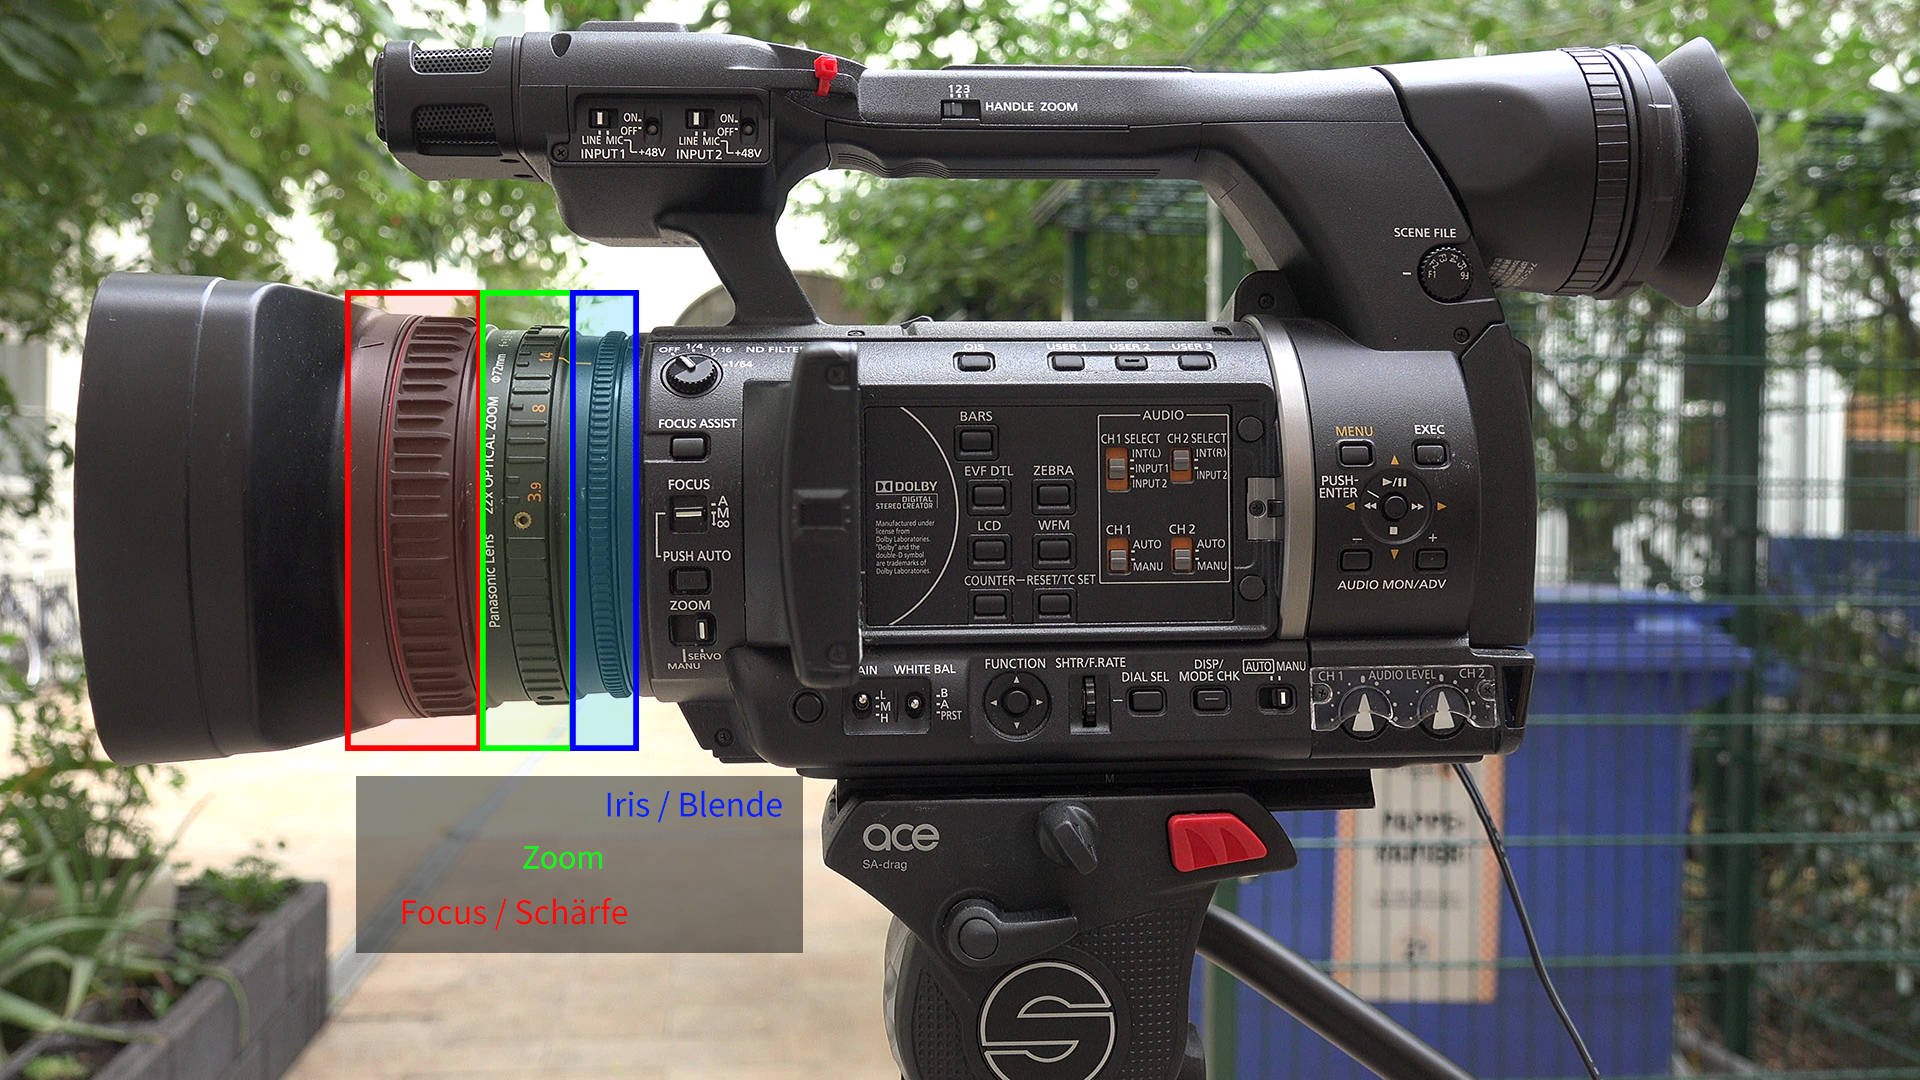
\includegraphics[width=0.9\textwidth]{images/panasonic-side-annotated.jpg}
		\caption{Panasonic Cam}
	\end{figure}
		\column{0.5\textwidth}
		Cameras are in manual mode because of difficult lighting situation.
		\begin{description}
			\item[Left Ring/red] Focus - control sharpness of the image.
			\item[Middle Ring/green] Zoom - vary the focal length.
			\item[Right Ring/blue] Iris - will have to be adjusted throughout the day. If there is anything wrong, contact C3VOC helpdesk.
		\end{description}
	\end{columns}
\end{frame}

\begin{frame}{Zoom Control Panasonic}
	\begin{columns}[T,onlytextwidth]
		\column{0.5\textwidth}
	\begin{figure}
		\centering
		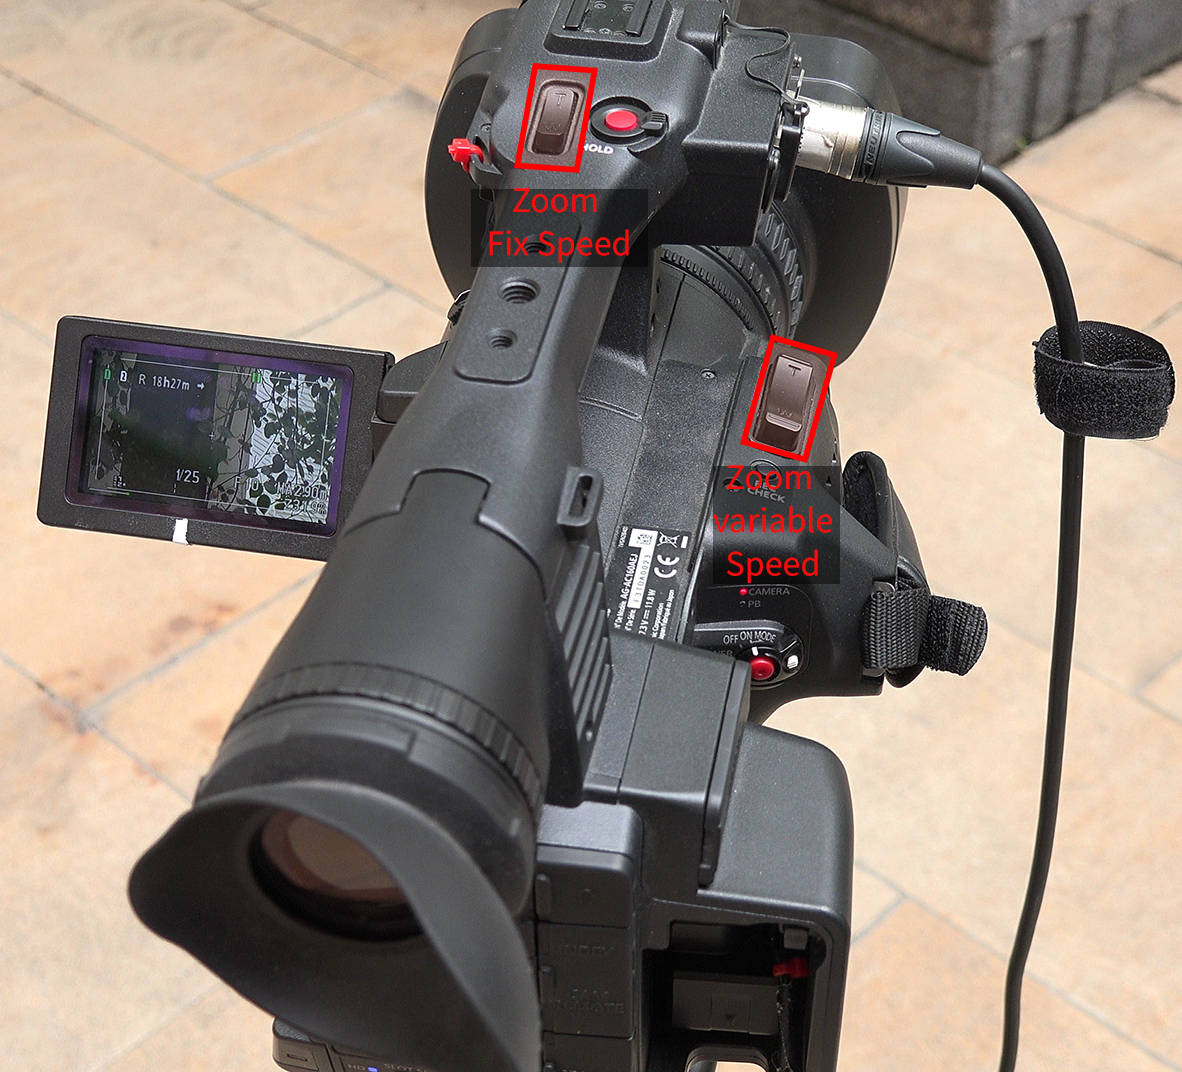
\includegraphics[width=0.99\textwidth]{images/panasonic-zoom-annotated.jpg}
		\caption{Panasonic Cam}
	\end{figure}
		\column{0.5\textwidth}
		\begin{itemize}
			\item For smooth zoom use the zoom buttons.
			\item Gentle touch $\Rightarrow$ slow zoom
			\item Top Buttons fixed speed
		\end{itemize}
	\end{columns}
\end{frame}

\begin{frame}{Display Indicators Panasonic}
	\begin{columns}[T,onlytextwidth]
		\column{0.5\textwidth}
	\begin{figure}
		\centering
		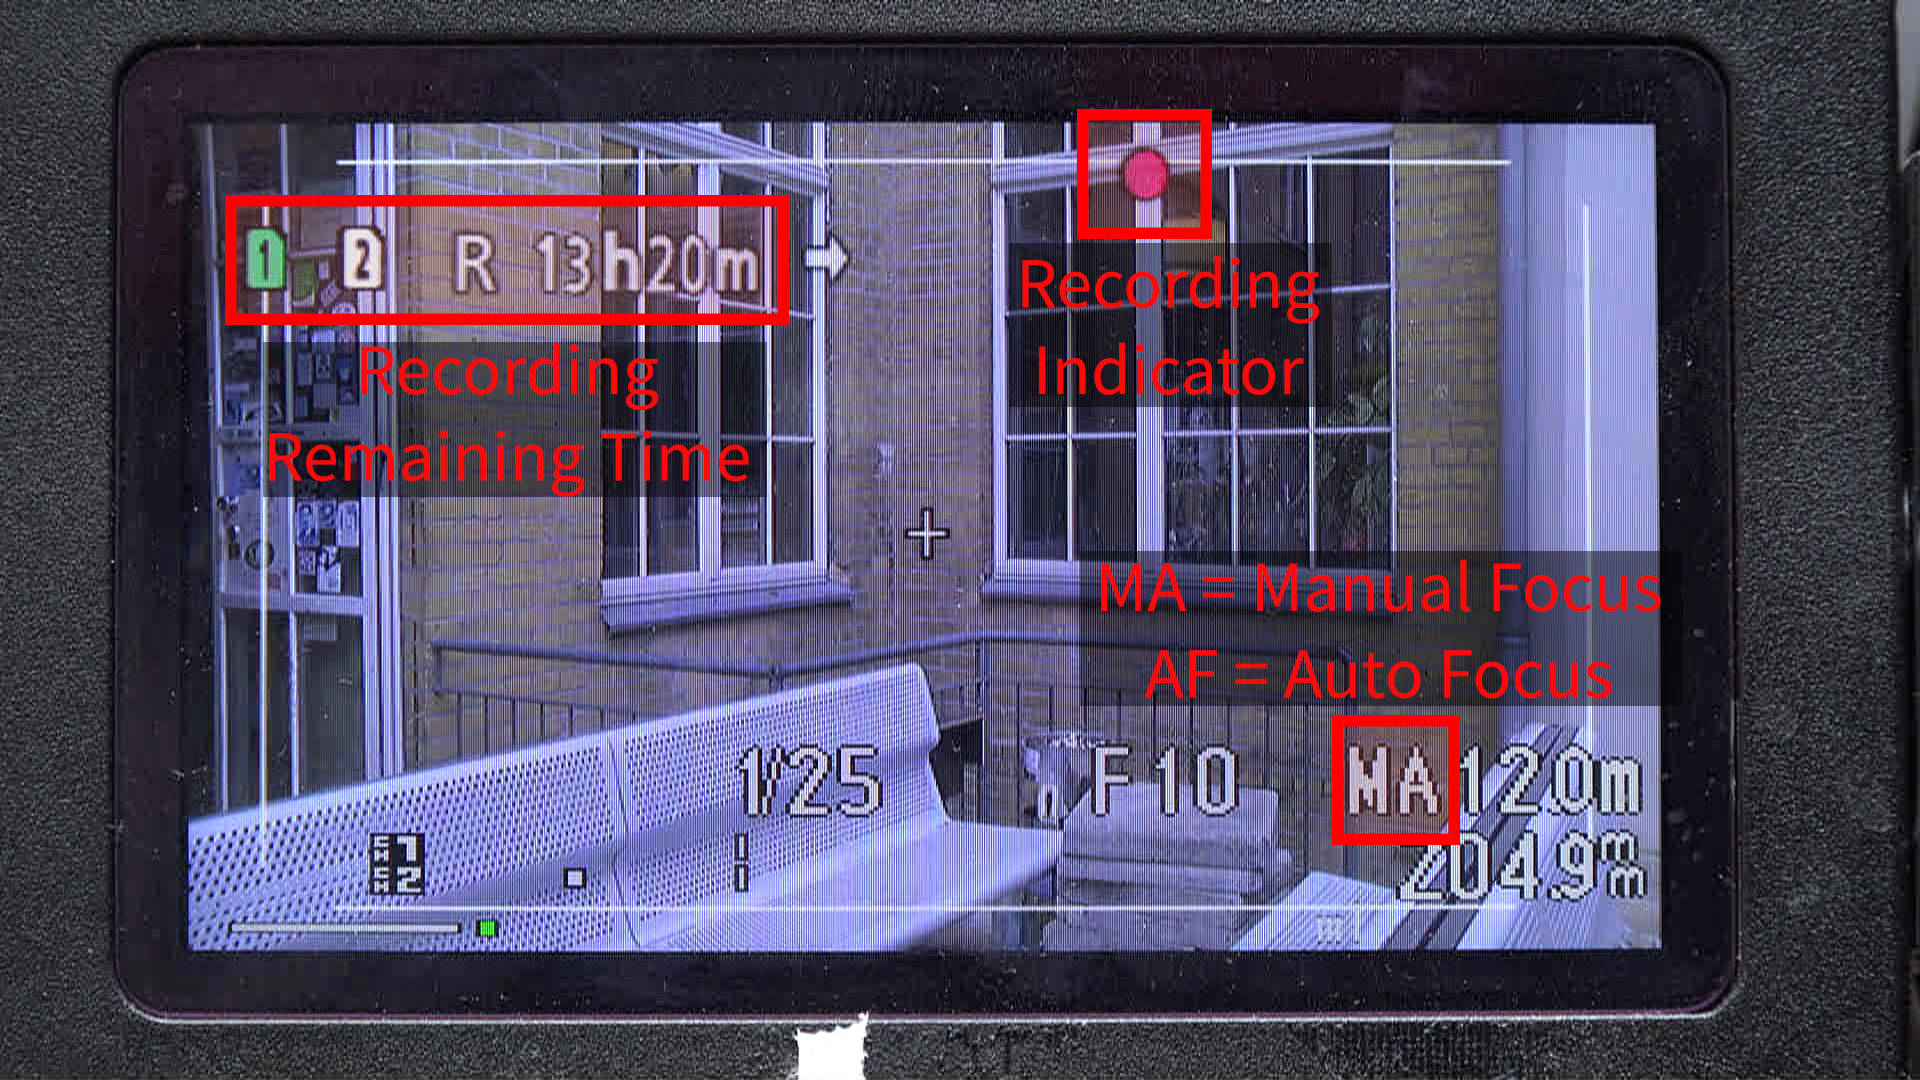
\includegraphics[width=0.9\textwidth]{images/panasonic-display-annotated.jpg}
		\caption{Panasonic Display Indicators}
	\end{figure}
		\column{0.5\textwidth}
		\begin{description}
			\item[Rec Indicator] The recording must always run, even during the break.
			\item[Focal Indicator] Use only manual focus!
			\item[Remaining Time] It must have enough remaing time before talk.
		\end{description}
		\metroset{block=fill}
		\begin{alertblock}{Alert}
			Alert the A/V-Technician if something's wrong.
		\end{alertblock}
	\end{columns}
\end{frame}

% !TEX root = ../main.tex

\begin{frame}{Hardware Camera Controls Sony PXW-Z200}
	\begin{columns}[T,onlytextwidth]
		\column{0.5\textwidth}
	\begin{figure}
		\centering
		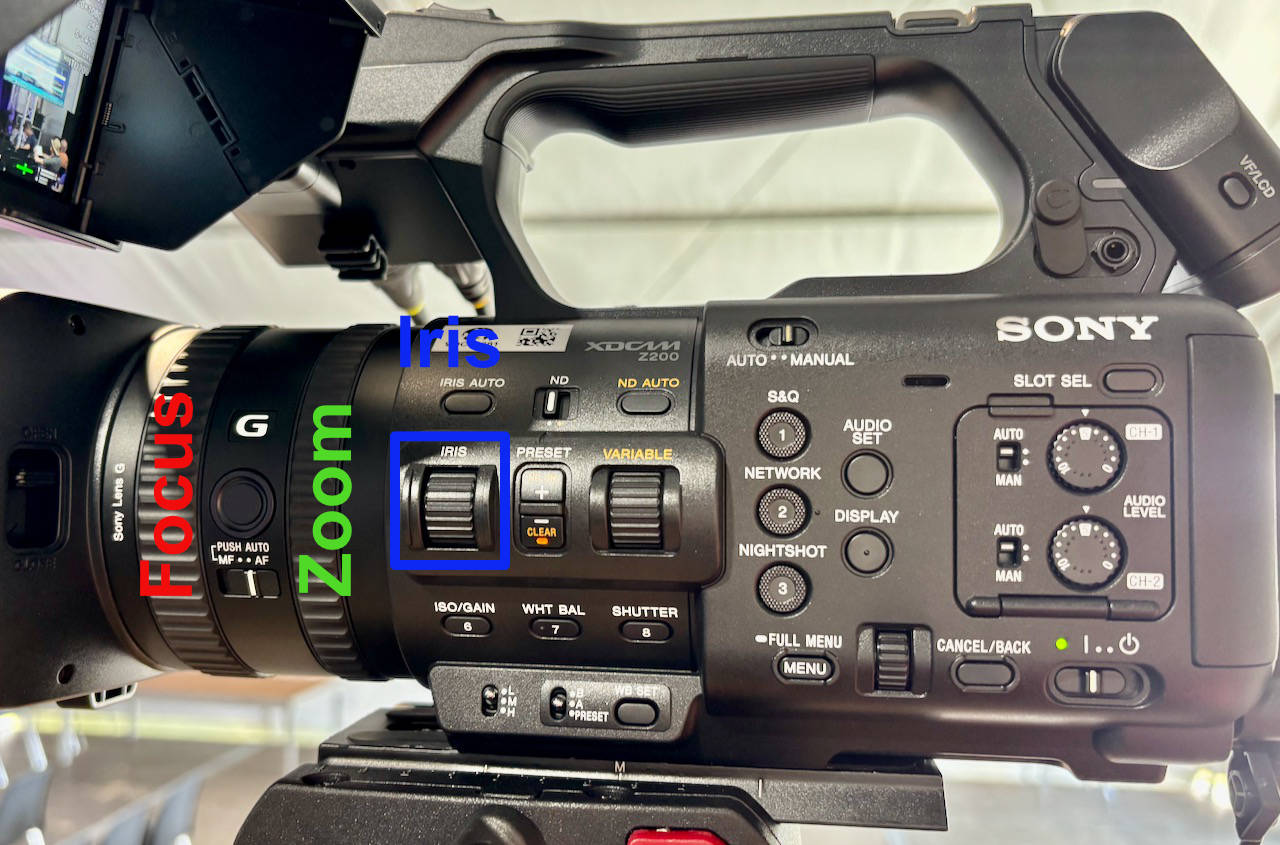
\includegraphics[width=0.9\textwidth]{images/sony-side-annotated.jpg}
		\caption{Sony Cam}
	\end{figure}
		\column{0.5\textwidth}
		Cameras are in manual mode because of difficult lighting situation.
		\begin{description}
			\item[Left Ring/red] Focus - control sharpness of the image.
			\item[MF/AF Selector] Auto Focus - always on.
			\item[Middle Ring/green] Zoom - vary the focal length.
			\item[Right Ring/blue] Iris - adjust according to lighting situation.
		\end{description}
	\end{columns}
  If there is anything wrong, contact C3VOC helpdesk.
\end{frame}

\begin{frame}{Zoom Control Sony}
	\begin{columns}[T,onlytextwidth]
		\column{0.5\textwidth}
	\begin{figure}
		\centering
		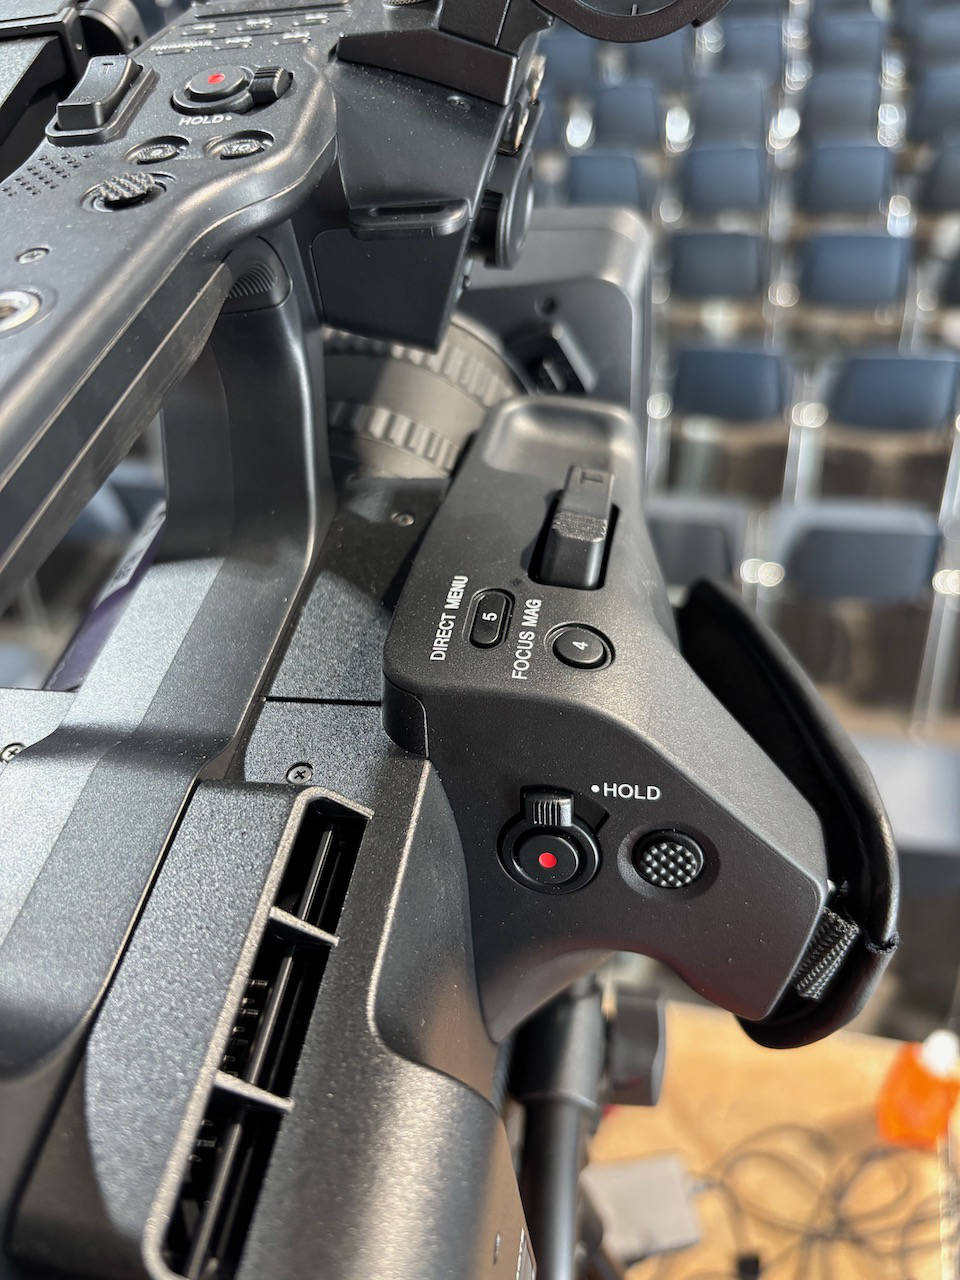
\includegraphics[width=0.99\textwidth]{images/sony-zoom.jpg}
		\caption{Sony Cam}
	\end{figure}
		\column{0.5\textwidth}
		\begin{itemize}
			\item For smooth zoom use the zoom buttons.
			\item Gentle touch $\Rightarrow$ slow zoom
		\end{itemize}
	\end{columns}
\end{frame}

\begin{frame}{Display Indicators Sony}
	\begin{columns}[T,onlytextwidth]
		\column{0.5\textwidth}
	\begin{figure}
		\centering
		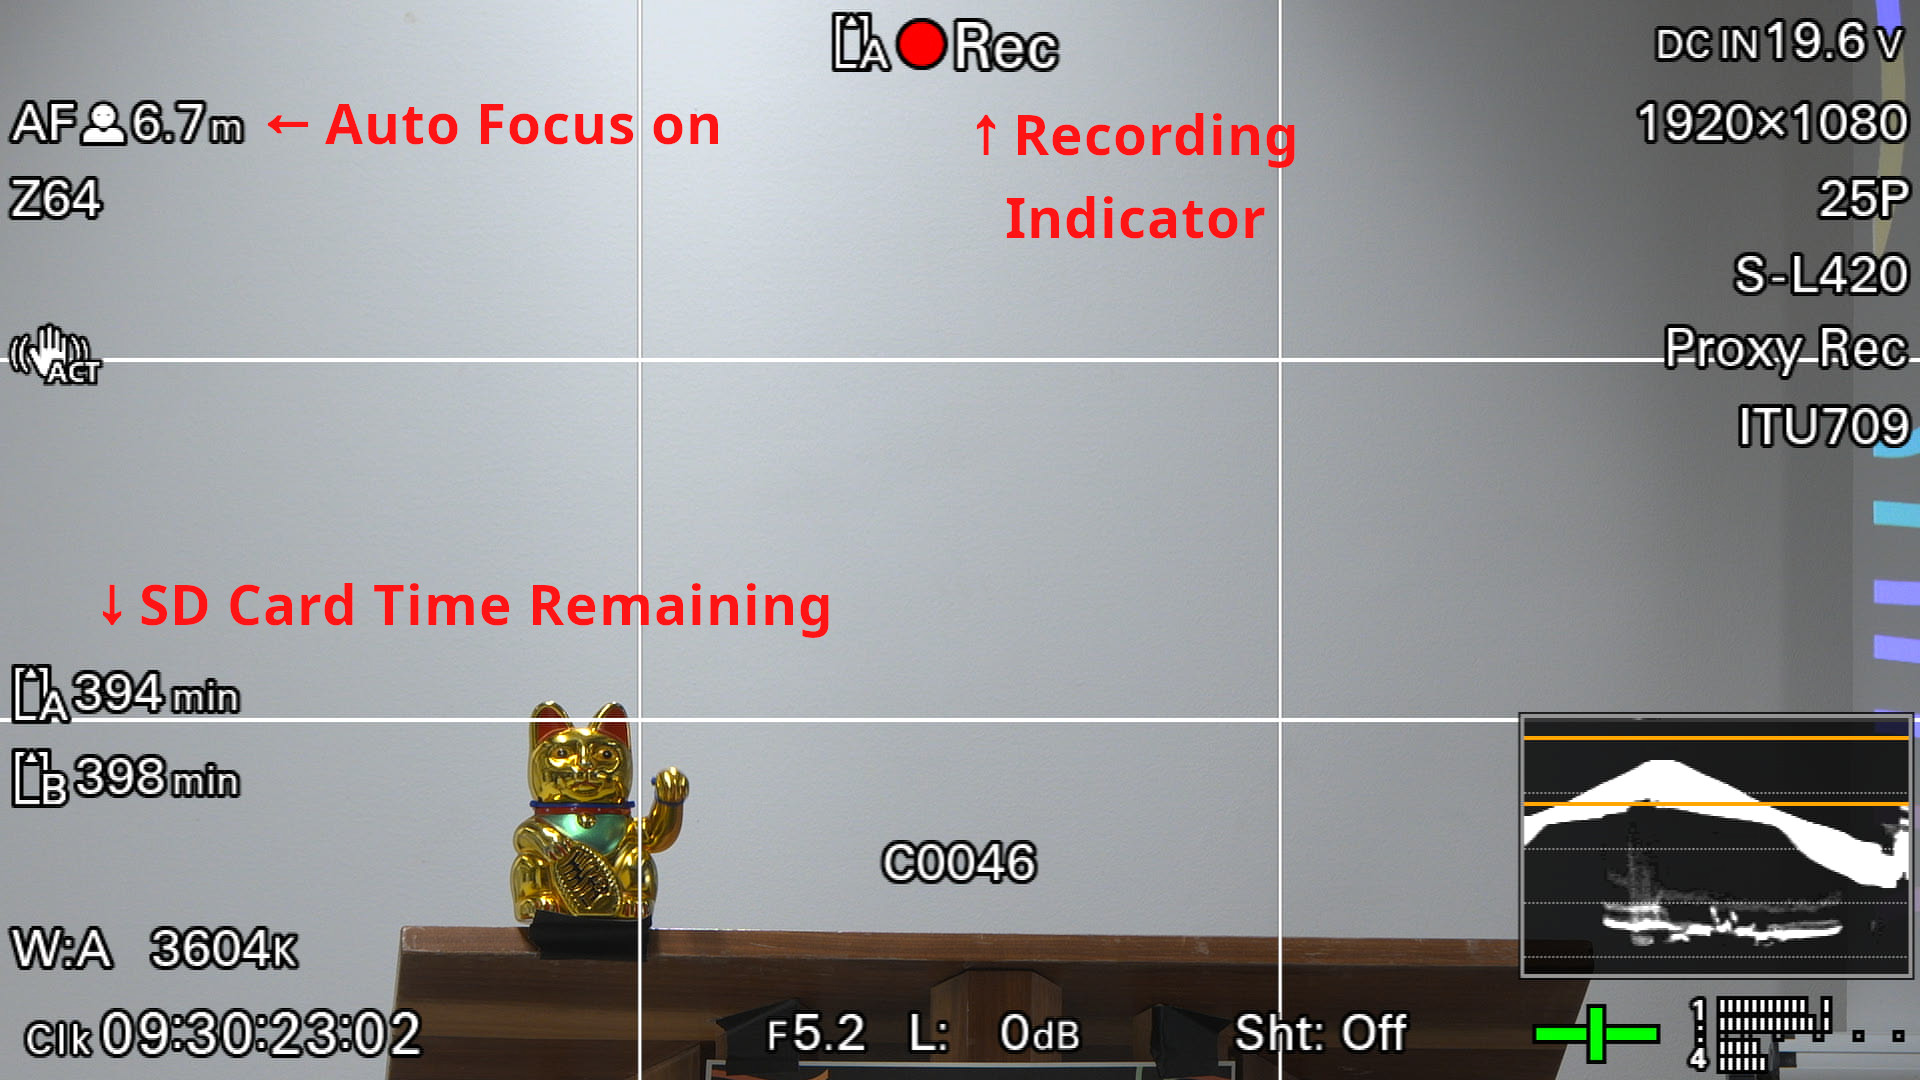
\includegraphics[width=0.9\textwidth]{images/sony-display-description.jpg}
		\caption{Sony Display Indicators}
	\end{figure}
		\column{0.5\textwidth}
		\begin{description}
			\item[Focal Indicator] Autofocus with face tracking is awesome!
			\item[Rec Indicator] The recording must always run, even during the break.
			\item[Remaining Time] More minutes remaining than the length of the next talk.
		\end{description}
		\metroset{block=fill}
		\begin{alertblock}{Alert}
			Alert the A/V-Technician if something's wrong.
		\end{alertblock}
	\end{columns}
\end{frame}

% % !TEX root = ../main.tex

\begin{frame}{Hardware Camera Controls JVC}
	\begin{columns}[T,onlytextwidth]
		\column{0.5\textwidth}
	\begin{figure}
		\centering
		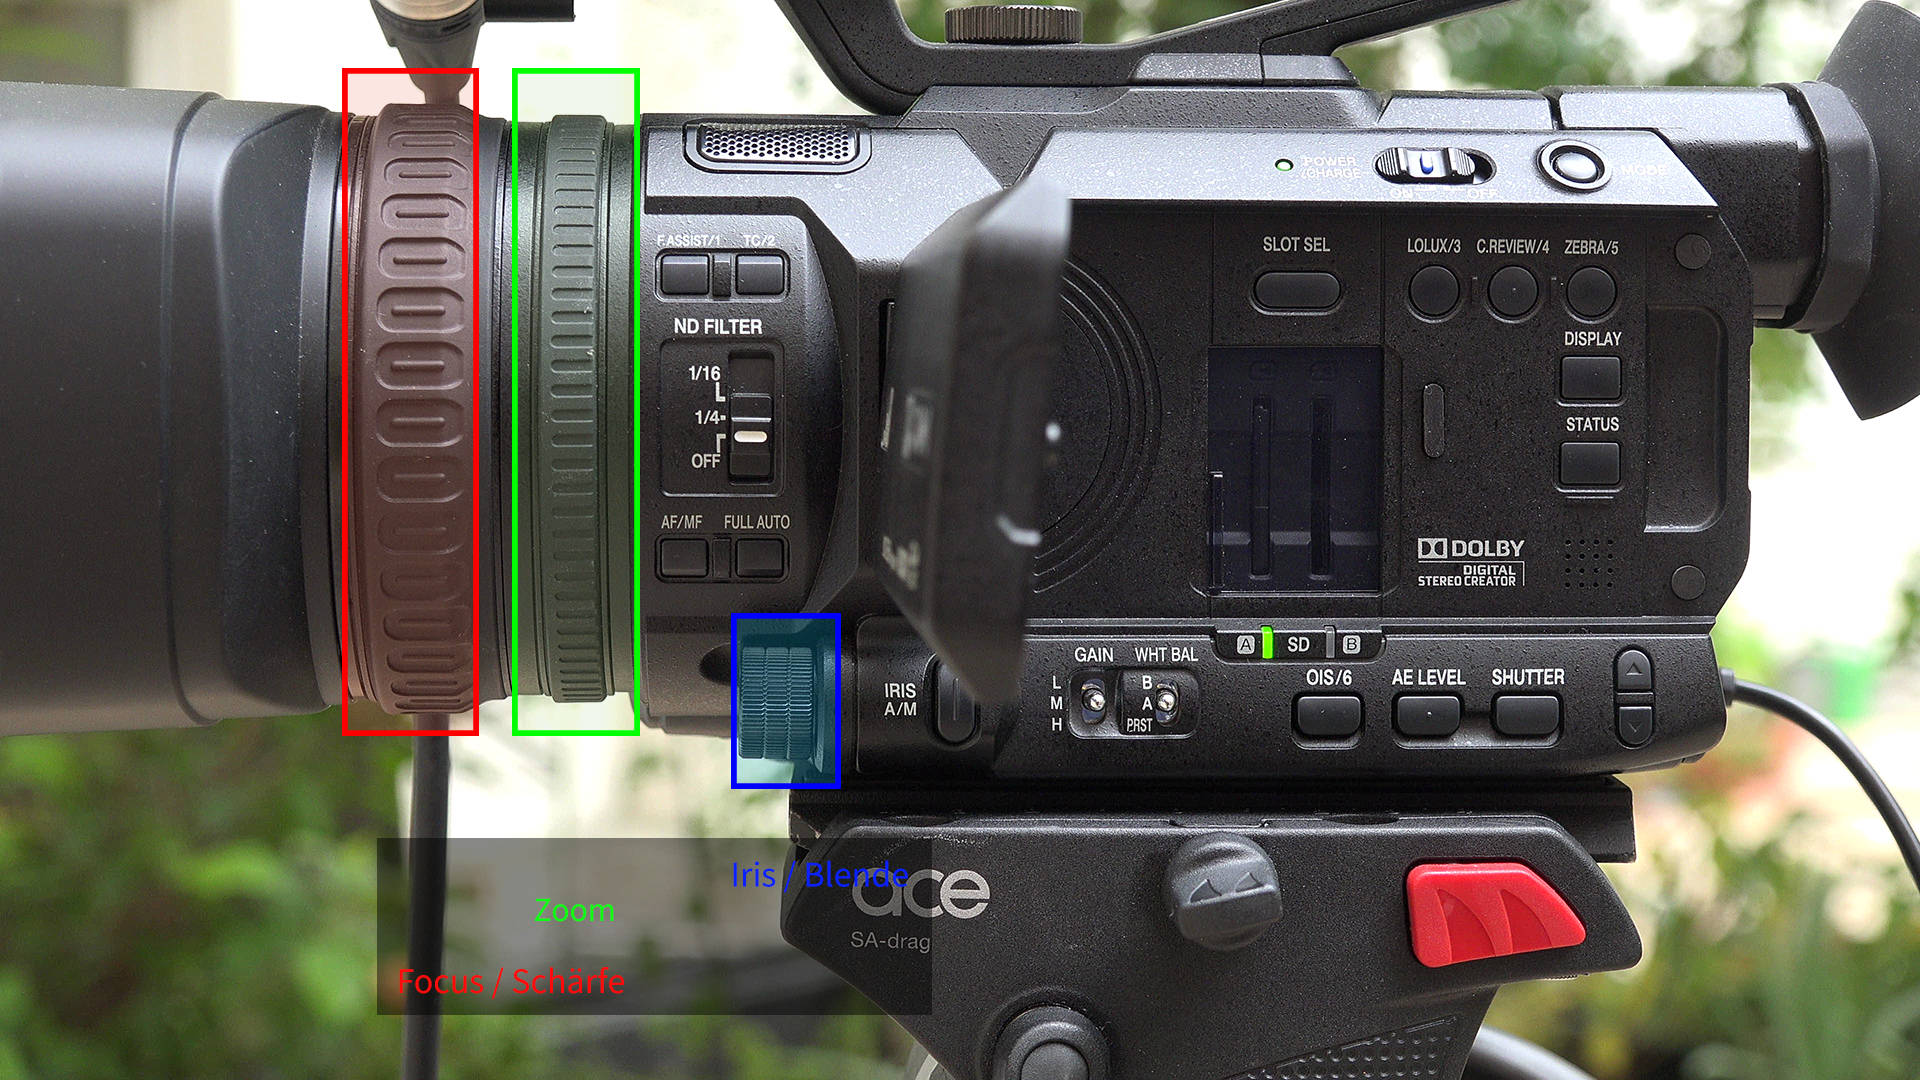
\includegraphics[width=0.9\textwidth]{images/jvc-side-annotated.jpg}
		\caption{JVC Cam}
	\end{figure}
		\column{0.5\textwidth}
		Cameras are in manual mode because of difficult lighting situation.
		\begin{description}
			\item[Left Ring/red] Focus - control sharpness of the image.
			\item[Middle Ring/green] Zoom - vary the focal length.
			\item[Right Ring/blue] Iris - will have to be adjusted throughout the day. For lighting issues talk to the A/V tech via intercom.
		\end{description}
	\end{columns}
\end{frame}

\begin{frame}{Zoom Control JVC}
	\begin{columns}[T,onlytextwidth]
		\column{0.5\textwidth}
	\begin{figure}
		\centering
		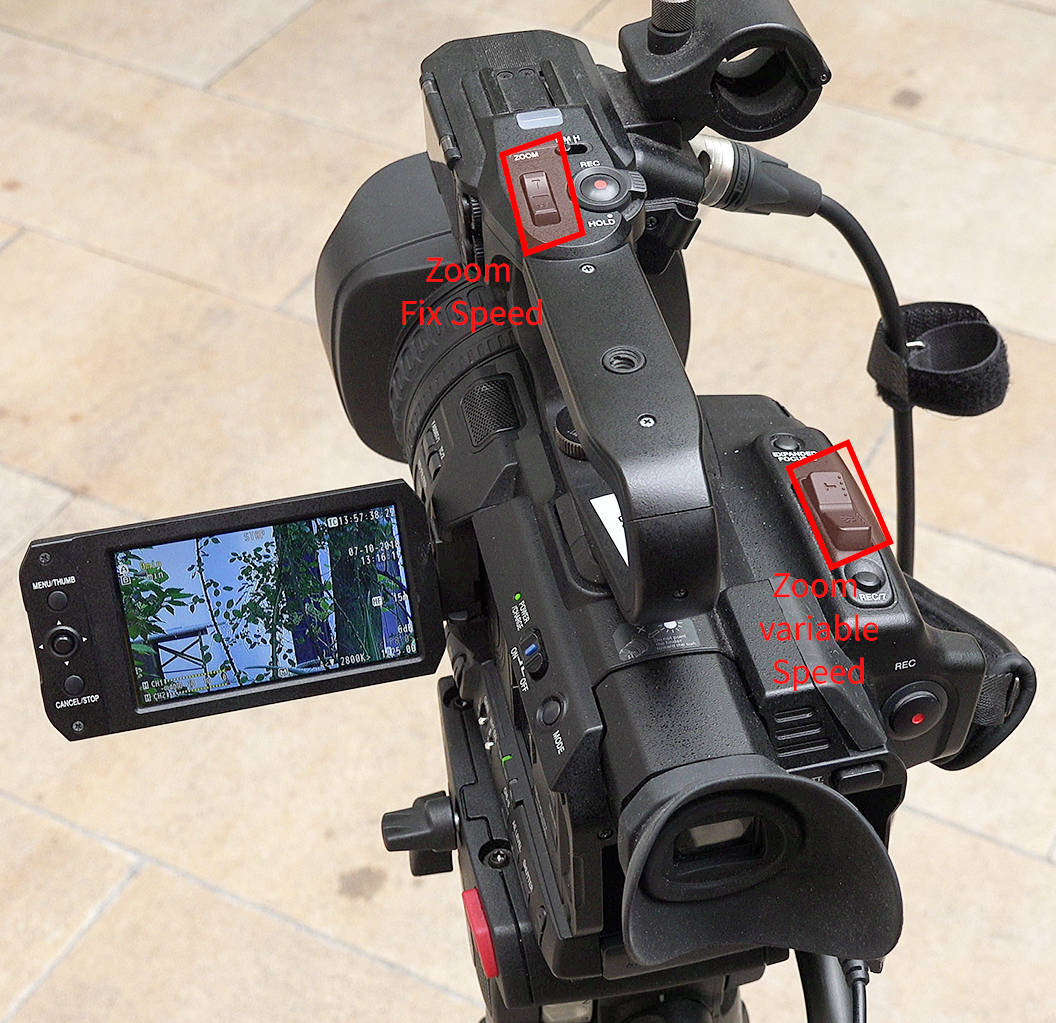
\includegraphics[width=0.9\textwidth]{images/jvc-zoom-annotated.jpg}
		\caption{JVC Cam}
	\end{figure}
		\column{0.5\textwidth}
		\begin{itemize}
			\item For smooth zoom use the zoom buttons.
			\item Gentle touch $\Rightarrow$ slow zoom
			\item Top Buttons fixed speed
		\end{itemize}
	\end{columns}
\end{frame}

\begin{frame}{Display Indicators JVC}
	\begin{columns}[T,onlytextwidth]
		\column{0.5\textwidth}
	\begin{figure}
		\centering
		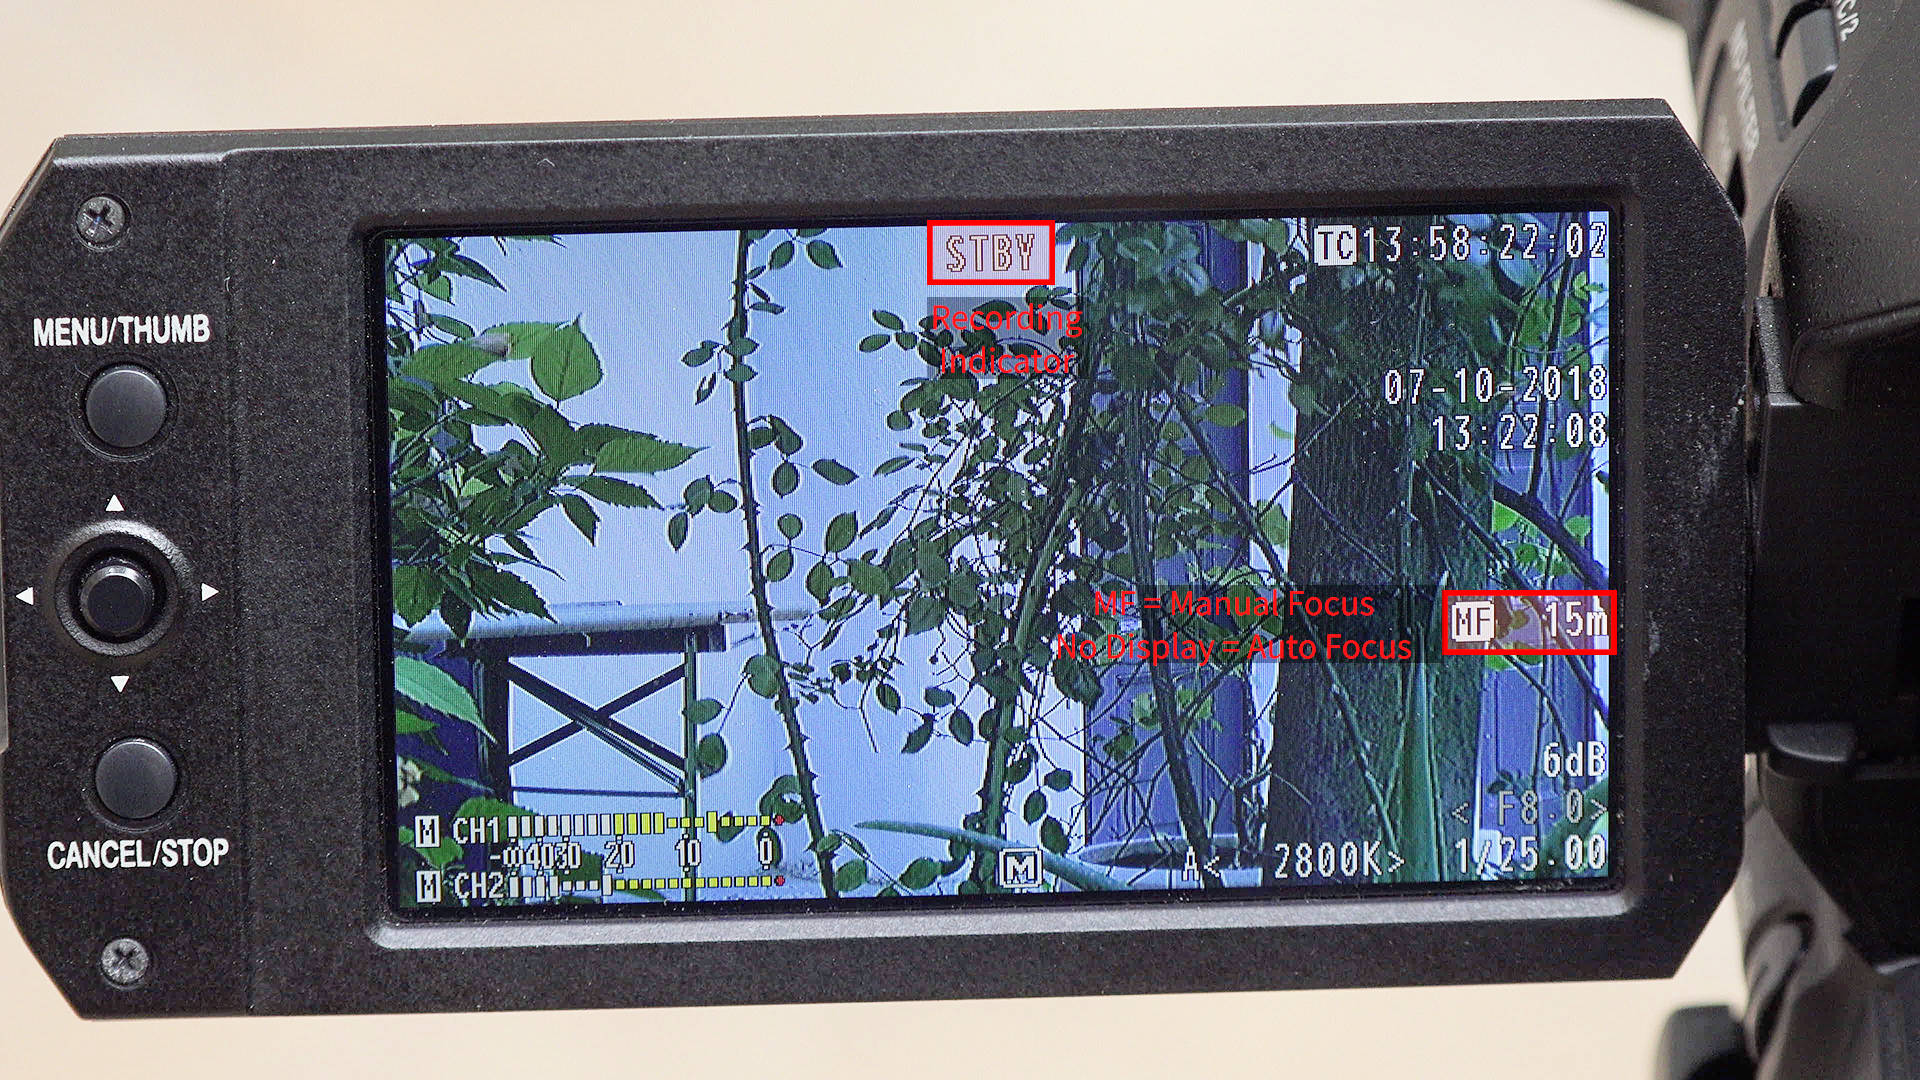
\includegraphics[width=0.9\textwidth]{images/jvc-display-annotated.jpg}
		\caption{Panasonic Display Indicators}
	\end{figure}
		\column{0.5\textwidth}
		\begin{description}
			\item[Rec Indicator] The recording must always run, even during the break.
			\item[Focal Indicator] Use only manual focus!
		\end{description}
		\metroset{block=fill}
		\begin{alertblock}{Alert}
			Alert the A/V-Technician if something's wrong.
		\end{alertblock}
	\end{columns}
\end{frame}

% !TEX root = ../main.tex

%\begin{frame}{Tripod Handle Controls}
%	\begin{columns}[T,onlytextwidth]
%	\column{0.5\textwidth}
%	\begin{figure} 
%		\centering
%		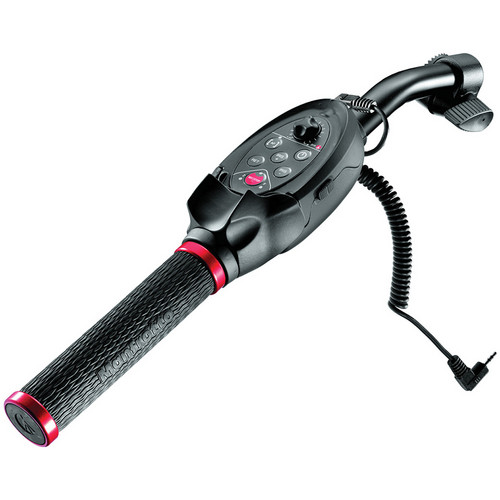
\includegraphics[width=0.7\textwidth]{images/tripod-handle.jpeg}
%		\caption{Tripod Handle}
%	\end{figure}
%
%	\column{0.5\textwidth}
%	Beware: various models in use.
%	\begin{description}
%		\item[Zoom Control] lever above red ring
%		\item[Red Button] Start/stop recording, don't touch
%		\item[Other Buttons] markings on the handle
%   \end{description}
%	\end{columns}
%\end{frame}

\begin{frame}{Tripod}
	\begin{columns}[T,onlytextwidth]
	\column{0.4\textwidth}
	\begin{figure} 
		\centering
		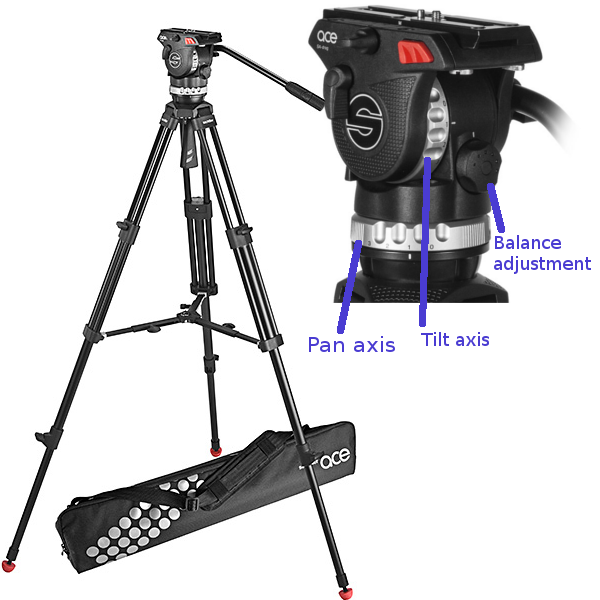
\includegraphics[width=0.9\textwidth]{images/tripod-complete.png}
		\caption{Tripod}
	\end{figure}
	
	\column{0.6\textwidth}
	\begin{itemize}
			\item Should be level - check the water bubble.
			\item Variable brakes - can be adjusted to your needs.
			\item Tilt axis should be balanced, so that the camera doesn't tilt up or down on its own.
			\item Pan axis is needed all of the time. Set it so you can do smooth pans all over the stage.
		\end{itemize}
		\metroset{block=fill}
		\begin{alertblock}{Alert}
			Alert the A/V-Technician if something's wrong or misplaced.
		\end{alertblock}
	\end{columns}
\end{frame}

\begin{frame}{SD-Card Recording}
		\begin{itemize}
			\item Two SD-Cards in every Camera
			\item Backup Recording
			\item Turn on Recording before first shift in the morning -> Red Dot somewhere in the Display.
			\item Control Recording Time remaining. 
		\end{itemize}
		\metroset{block=fill}
		\begin{alertblock}{Alert}
			Alert the A/V-Technician if something's wrong or not running.
		\end{alertblock}
\end{frame}


\section{Next Steps}
\begin{frame}{Hands-On Training}
	\begin{itemize}
		\item Please do hands-on training!
		\begin{itemize}
			\item The only way to get proficient with the tripod is to feel it
			\item Feel free to try things in a break between talks
		\end{itemize}
		\item VOC A/V-Techs are there to help you
	\end{itemize}
\end{frame}


\end{document}
